\chapter{上田の研究をもっと引用してもらう手法の開発}\label{chap:method}

ここに書いてある方法を使えば、秒速で秒速で1億円稼ぐ男になれます。なれません。


\section{手法の概要}

図に書くと図\ref{fig:vq_map_128part}っていう感じ。
式で書くとだいたい以下のような感じになるんじゃないんかなー。
式(\ref{eq:j})が肝。

\begin{figure}[h]
        \begin{center}
        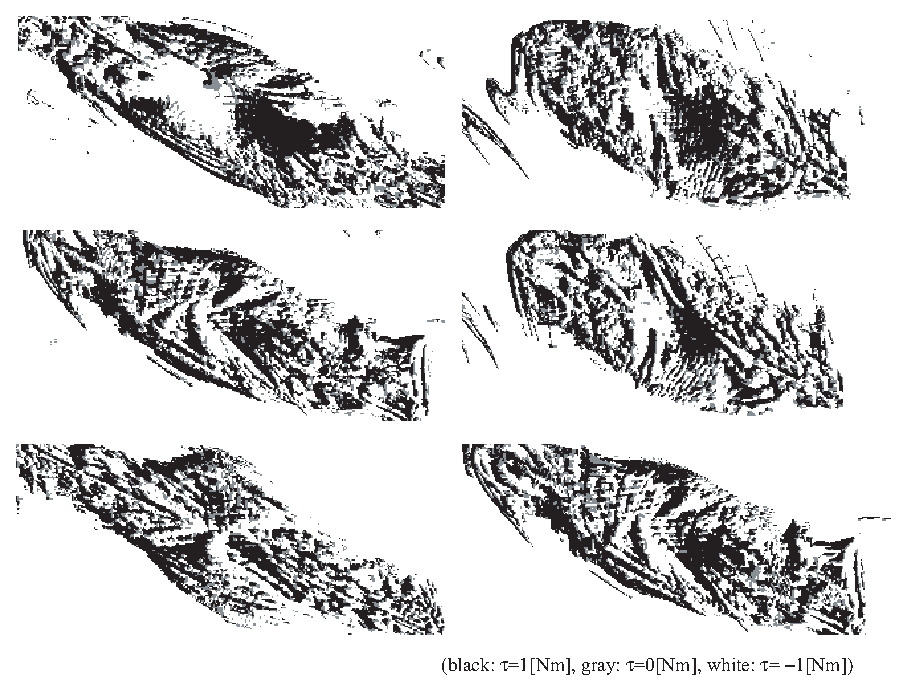
\includegraphics[width=1.0\linewidth]{figs/vq_map_128part.eps}
        \caption{Representative Vectors of the $N_c = 128$ Map}
        \label{fig:vq_map_128part}
        \end{center}
\end{figure}




\begin{align}
s_0, a(t_0), s(t_1), a(t_1), s(t_2), a(t_2), \dots, a(t_{T-1}), s_\text{f} \quad (s_0 = s(t_0), s_\text{f} = s(t_T)). 
\end{align}
\begin{align}
& s_0, \pi(s_0), s(t_1), \pi(s(t_1)), s(t_2), \pi(s(t_2)), \dots, \pi(s(t_{T-1})), s_\text{f}
\end{align}
\begin{align}
\pi &: \mathcal{S} \to \mathcal{A} \label{eq:policy_state_action_sequence}
\end{align}
\begin{align}
\mathcal{S} &= \{s_i | i=0,1,2,\dots,N-1 \}, \text{ and} \\
\mathcal{A} &= \{a_j | j=0,1,2,\dots,M-1 \}
\end{align}
\begin{align}
\pi : \mathcal{S} - \mathcal{S}_\text{f} \to \mathcal{A}. \label{eq:policy}
\end{align}
\begin{align}
\dot{\V{x}}(t) &= \V{f}[\V{x}(t),\V{u}(t)], \quad \V{x}(0) = \V{x}_0, \quad t \in [0,t_\text{f}].\label{eq:system} \\
&  \nonumber 
\end{align}
\begin{align}
g[\V{x}(t), \V{u}(t)] \in \Re \quad (t \in [0,t_\text{f}]). \label{eq:evaluation_function}
\end{align}
\begin{align}
J[\V{u}] = \int_{0}^{t_\text{f}} g[\V{x}(t), \V{u}(t)] dt + V(\V{x}_\text{f}).  \label{eq:functional}
\end{align}
\begin{align}
\max_{\V{u}:[0,t_\text{f}) \to \Re^m} J[\V{u};\V{x}_0].  \label{eq:optimal_control_problem}
\end{align}
\begin{align}
\V\pi^*: \Re^n \to \Re^m
\end{align}
\begin{align}
\max_{\V{u}:[0,t_\text{f}) \to \Re^m} J[\V{u};\V{x}_0] &= \max_{\V{u}:[0,t') \to \Re^m} \int_{0}^{t'} g[\V{x}(t), \V{u}(t)] dt \nonumber \\ &+ \max_{\V{u}:[t',t_\text{f}) \to \Re^m} \int_{t'}^{t_\text{f}} g[\V{x}(t), \V{u}(t)] dt + V(\V{x}_\text{f}) \nonumber \\
	&= \max_{\V{u}:[0,t') \to \Re^m} \int_{0}^{t'} g[\V{x}(t), \V{u}(t)] dt + \max_{\V{u}:[t',t_\text{f}) \to \Re^m} J[\V{u};\V{x}(t')]. \label{eq:j}
\end{align}
\begin{align}
V^{\V\pi}(\V{x}) &= J[\V{u};\V{x}], \label{eq:def_of_value} \\
&\text{ where } \V{u}(t) = \V\pi(\V{x}(t)), \ 0\le t \le t_\text{f}. \nonumber 
\end{align}
\begin{align}
\mathcal{P}_{ss'}^a &= P[s(t_{i+1}) = s' | s(t) = s,a(t) = a], \label{eq:state_transition}\\
&(\forall t \in \{t_0,t_1,\dots,t_{T-1}\}, \forall s \in \mathcal{S} - \mathcal{S}_\text{f}, \text{ and } \forall s' \in \mathcal{S}). \nonumber
\end{align}
\begin{align}
\mathcal{R}_{ss'}^a \in \Re
\end{align}
\begin{align}
J[a;s(t_0)] = J[a(0),a(1),\dots,a(t_{T-1})] = \sum_{i=0}^{T-1} \mathcal{R}_{s(t_i)s(t_{i+1})}^{a(t_i)} + V(s(t_T)),
\end{align}
\begin{align}
\max J[a;s(t_0)]. 
\end{align}
\begin{align}
J^{\V{\pi}} = \int_\mathcal{X} p(\V{x}_0) J[\V{u};\V{x}_0] d\V{x}_0 \quad\Big(\V{u}(t) = \V\pi(\V{x}(t))\Big),\label{eq:eval_general}
\end{align}
\begin{align}
\dfrac{\partial V(\V{x})}{\partial t} = \max_{\V{u}\in\mathcal{U}} \left[g[\V{x},\V{u}] + \dfrac{\partial V(\V{x})}{\partial\V{x}} \V{f}[\V{x},\V{u}] \right].\label{eq:hjb}
\end{align}
\begin{align}
U_\text{att}(\V{x}) = \dfrac{1}{2} \xi \rho^2 (\V{x})
\end{align}
\begin{align}
U_\text{rep}(\V{x}) =
\begin{cases}
\dfrac{1}{2}\eta \left( \dfrac{1}{\rho(\V{x})} - \dfrac{1}{\rho_0} \right)^2 &\text{if } \rho(\V{x}) \le \rho_0, \\
0 &\text{if } \rho(\V{x}) > \rho_0,
\end{cases}
\end{align}
\begin{align}
U(\V{x}) = U_\text{att}(\V{x}) + U_\text{rep}(\V{x})
\end{align}
\begin{align}
\V{F}(\V{x}) &= - (\partial U/\partial x_1,\partial U/\partial x_2,\dots,\partial U/\partial x_n)^T \nonumber \\
&= -\nabla U({\V{x}}). 
\end{align}
\begin{align}
V(\V{x};\theta_1,\theta_2,\dots,\theta_{N_\theta}) \nonumber
\end{align}
\begin{align}
\phi_i(\V{x}) &= \exp \left\{-\dfrac{1}{2}(\V{x} - \V{c}_i)^t M_i (\V{x} - \V{c}_i) \right\},
\end{align}
\begin{align}
b_i(\V{x}) &= \dfrac{\phi_i(\V{x})}{\sum_{j=1}^{N_\phi} \phi_j(\V{x})}, \ (N_\phi: \text{ number of RBFs in the space})
\end{align}
\begin{align}
V(\V{x}) &= \sum_{i=1}^{N_\phi} \nu_i b_i(\V{x}). \label{eq:rbf_weighted_sum}
\end{align}
\begin{align}
\phi_i(x) &= \exp \left\{-\dfrac{1}{2}(x - i)^2 \right\} \nonumber
\end{align}

\begin{align}
V(\V{x}) = \sum_{i=0}^3 w_i V(\V{x}_i)
\end{align}


\begin{table}[htbp]
        \begin{center}
	\caption{謎のパラメータ}
        \label{table:parameter_value}
\begin{footnotesize}
\begin{minipage}{12em}
        \begin{tabular}{c|rl}
\multicolumn{3}{c}{(a)}\\
        \thline
parameter & \multicolumn{2}{c}{value} \\
        \hline
$\ell_1,\ell_2$ & 1.0&[m] \\
$\ell_{c1},\ell_{c1}$ & 0.50&[m] \\
$m_1,m_2$ & 1.0&[kg] \\
$I_1,I_2$ & 1.0&[kg m$^2$] \\
$g$ & 9.8&[m/s$^2$] \\
   \thline
  \end{tabular}
\end{minipage}
\hspace{2em}
\begin{minipage}{12em}
        \begin{tabular}{c|l}
\multicolumn{2}{c}{(b)}\\
        \thline
variable & domain \\
        \hline
$\theta_1$ & $(-\infty,\infty)$ \\
$\theta_2$ & $(-\infty,\infty)$ \\
$\dot\theta_1$ & $[-720,720]$[deg/s] \\
$\dot\theta_2$ & $[-1620,1620]$[deg/s] \\
\hline
$\tau$ & $-1,0,$ or $1$[Nm] \\
   \thline
  \end{tabular}
\end{minipage}
\end{footnotesize}
  \end{center}
\end{table}


